\subsection{\headershortacr{QoE} Study for Typical User Scenarios}\label{sec:application:qoe_user_behaviour:typical_user_scenarios}

\subsubsection*{Watch later Scenario}\label{sec:application:qoe_user_behaviour:typical_user_scenarios:watch_later}
In the \watchLater scenario, a user requests a video, but the user does not expect that the video playout starts immediately. 
This may be the case for example when the user wants to watch an HD at a later time and expects low network bandwidth is low. 
During that initial delay, the user may opt do something else, e.g. opening another web page in a parallel tab in the browser.
Thus, \gls{QoE} is not affected by initial delays and we only need to consider \(Q_1\) in \refeq{eq:application:qoe_user_behaviour:typical_user_scenarios:youtube_qoe:stalling:parameterized_model}.

In the steady state, we have \(L=\frac{d}{\lambda}\) and \(N^*=\frac{\mu-\lambda}{d}\) and we obtain the following QoE relation in \refeq{eq:application:qoe_user_behaviour:typical_user_scenarios:stalling_steady_state}. 

\begin{equation}
   Q_1(L,N^*) = e^{\left(\mu-\lambda\right)(\frac{\alpha}{\lambda} +\frac{\beta}{d^*})}
	 = e^{-\alpha \frac{1-a}{a} - \beta \frac{1-a}{d^*}}
\label{eq:application:qoe_user_behaviour:typical_user_scenarios:stalling_steady_state}
\end{equation}

Since the \gls{QoE} function in \refeq{eq:application:qoe_user_behaviour:typical_user_scenarios:stalling_steady_state} is strictly monotonically increasing in the normalized buffer size \(d^*\), the optimum is achieved for 
\[Q_+=\lim\limits_{d^* \to \infty} Q_1(L,N^*)=e^{-\alpha \frac{1-a}{a}}.\]
Thus, the QoE value only depends on the parameter \(\alpha\) in the limit.
To see for which buffer size we are close to the optimum, we consider the relative difference \(\frac{Q_+-Q_1(L,N^*)}{Q_+}\) when it is less than \(\Omega=\SI{5}{\percent}\).
This is true for any \(d^*> -\beta \frac{1-a}{\log\left(1-\Omega\right)}\). 

For \(\beta \in \{0.05,0.2\}\), a small buffer size of \(d^*>\SI{4}{\second}\) is already sufficient to be close to the optimum \(Q_+\) for any offered network condition \(a\).
For users extremely sensitive to stalling, e.g. for \(\beta=0.8\), buffer sizes up to \SI{15}{\second} are required.
However, a buffer of \SI{4}{\second} is sufficient for a relative difference to the optimum of \SI{20}{\percent}. 
In general, the larger the buffer size the better the obtained \gls{QoE} is in this scenario. In practice, a buffer size of \SI{4}{\second} is a good choice.

\subsubsection*{Default Video Streaming Scenario}\label{sec:application:qoe_user_behaviour:typical_user_scenarios:default}

In the case of normal streaming, the user wants to watch a video immediately for a long period of time.
In contrast to the \watchLater scenario, the initial delay impacts the \gls{QoE} in the \watchNow scenario according to \refeq{eq:application:qoe_user_behaviour:typical_user_scenarios:youtube_qoe:combined:qsum}.

\begin{figure}
  \centering
  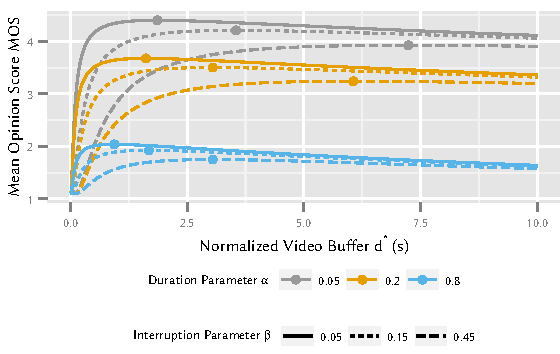
\includegraphics{application/qoe_user_behaviour/user_scenarios/figures/default_scenario}
  \caption{Dimensioning of buffer size in the \emph{Streaming Scenario} for available network bandwidth of \(a = 0.5\). Maxima marked as dots mainly depend on \(\beta\).}
  \label{fig:application:qoe_user_behaviour:typical_user_scenarios:default:default_scenario}
\end{figure}

\reffig{fig:application:qoe_user_behaviour:typical_user_scenarios:default:default_scenario} shows \gls{QoE} depending on the buffer size \(d^*\) for the \watchNow scenario and different user profiles in a network situation \(a=0.5\) leading to a stalling ratio \(R=0.5\).

Now, \gls{QoE} optima exist for finite buffer size, if the impact of the initial delay is taken into consideration. 
We notice that \(\alpha\) does increase the \gls{QoE} but has no significant impact on the optimal buffer size.
In contrast, for different \(\beta\) we observe different optima for the buffer size.
Therefore, we can neglect the interruption parameter \(\alpha\) when optimising the buffer size with regard to the \gls{QoE}.
A buffer size less than \SI{0.5}{\second} results in a severe loss of \gls{QoE} for all users.
A buffer size of \SIrange{2}{4}{\second} offers a good \gls{QoE} for the average user and any sensitive user.
Increasing the buffer size further decreases the \gls{QoE}.

\subsubsection*{Video Browsing Scenario}\label{sec:application:qoe_user_behaviour:typical_user_scenarios:browsing}

In the case of the \videoBrowsing scenario, the user watches a video for a short period of time. This includes cases such as, viewing a short video completely, viewing a short part of a long video or skipping ahead in a video frequently, thus watching multiple short parts of a video.
In this scenario, a steady state can not be assumed due to the short watching duration.
Since we know from the previous section that \(\alpha\) and \(\beta\) have only a marginal impact on the optimal \gls{QoE}, we consider only the default parameters \(\alpha=0.15\) and \(\beta=0.2\) in the following.
However, for video browsing, the impact of the initial delay may be more important for the user. Therefore, we consider two different types of delay sensitive users with \(\gamma=0.2\) as well as a more delay sensitive user with \(\gamma=0.8\).

\begin{figure}
  \centering
  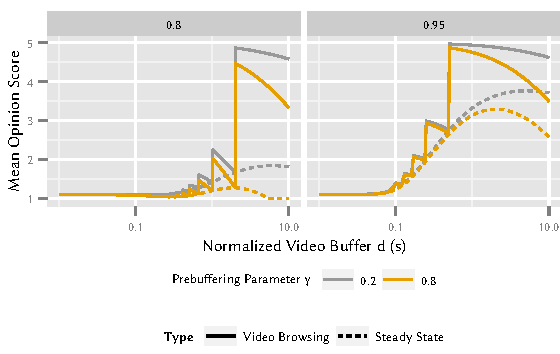
\includegraphics{application/qoe_user_behaviour/user_scenarios/figures/video_browsing}
  \caption{Dimensioning of buffers for \emph{Video Browsing} users with varying \gls{QoE} sensitivity to initial delays. Users abort the video after \SI{10}{\second}.}
  \label{fig:application:qoe_user_behaviour:typical_user_scenarios:browsing:video_browsing}
\end{figure}

In \reffig{fig:application:qoe_user_behaviour:typical_user_scenarios:browsing:video_browsing}, the impact of the buffer size on the \gls{QoE} is depicted for the case that the video is aborted after the first \SI{10}{\second} using a logarithmic x-axes. 
We consider two different network scenarios with an offered load of \(a = 0.8\) and \(a = 0.9\).
Multiple local QoE maxima exist independently of \(\gamma\), which appear when the number of stalling events change. 
For different values of \(\beta\) these maxima occur at the same buffer size.
Therefore, we can ignore \(\beta\) in this scenario. 
The local minima exist at the buffer size for which the last stalling event has the smallest possible length. 
The results for the steady state are also included and we observe that the steady state provides a lower bound for the finite buffer results.

Thus, the steady state can be used to perform worst case buffer dimensioning.
For very low offered loads \(a\), e.g. \(a = 0.1\), the \gls{QoE}'is very low for both, the steady state and the finite case. 
Thus, video streaming and especially \videoBrowsing is not desirable in this case. 
However, for larger buffer sizes, the difference between the local maxima and the steady state increases. 
Nevertheless, in those cases, the initial delay exceeds tens of seconds.
So this scenario can not be described as realistic \videoBrowsing.

In general, if the exact viewing length of a video was known, e.g. short videos will be watched completely, the buffer size could be set so that the \gls{QoE} lies at a local maximum which is independent of \(\gamma\).
However, this method can result in a severe loss of \gls{QoE}, depending on \(\gamma\) if the user aborts earlier, as the actual \gls{QoE} loss significantly depends on \(\gamma\). 
In practice, a buffer size of \SIlist{1;2}{\second} is recommended for video browsing. 
If the buffer size is set too large, \(\gamma\) determines again the actual \gls{QoE} loss.
For larger buffer sizes, the sensitivity \(\gamma\) to initial delays strongly influence the \gls{QoE}.